% Problem section - start here

% Number 790
% CAPMG Algebra Units 
% Delta x from v graph - CVPM, CAPM, NAPM
% JG

% Watermark
\AddToShipoutPicture*{\BackgroundPic}

\addtocounter {ProbNum} {1}

\begin{floatingfigure}[r]{.34\textwidth}
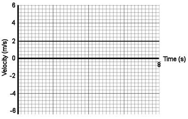
\includegraphics[scale=1]{/Users/jgates/desktop/latex/pics/vgraph3}
\end{floatingfigure}
 
{\bf \Large{\arabic{ProbNum}}} A velocity vs. time graph of a motion with constant velocity is shown at right.  Calculate the position of the object at $t =8~s$, assuming that it started at $x =7~m$. Show your work or explain your method. \paragraph{}
\noindent

\vfill
Calculate, as accurately as you can, the positions at $t =8~s$ of the objects whose velocity vs. time graphs are shown below, assuming that they each started at $x =7~m$. Show your work or explain your method.\paragraph{}
\noindent
\begin{figure}[ht]
\begin{minipage}[b]{0.5\linewidth}
\centering
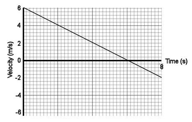
\includegraphics[scale=1]{/Users/jgates/desktop/latex/pics/vgraph4}
\end{minipage}
\hspace{0.5cm}
\begin{minipage}[b]{0.5\linewidth}
\centering
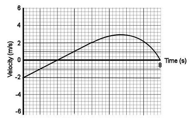
\includegraphics[scale=1]{/Users/jgates/desktop/latex/pics/vgraph5}
\end{minipage}
\end{figure}

\vfill
\vfill
\newpage
